% \documentclass[a4paper,11pt]{article}
% \usepackage[hyperref]{beamerarticle}

\documentclass[final]{beamer}

\usepackage{kotex}
\usepackage{amsfonts,amsmath,xob-amssymb}

\usepackage{amsthm}
\newtheorem{defn}{Definition}
\newtheorem{thm}{Theorem}

\usepackage{cancel}
\usepackage{enumerate}

\mode<presentation>{
	\usetheme{Madrid}
	\usecolortheme{default}
	\usefonttheme{professionalfonts}
}

\def\b{\boldsymbol}

\mode<article>{
\usepackage{fullpage}
}
\usepackage{ulem}

\author[조남운]{\url{econMath.namun+2016su@gmail.com}}
\title{Euclidean Spaces}
\subtitle{Ch.10}

\begin{document}
	
\maketitle

\mode<presentation>{
\begin{frame}[t]{Table of Contents}
	\tableofcontents
\end{frame}
%--- Next Frame ---%
}

\section{Points and Vectors in Euclidean Space} % (fold)
\label{sec:points_and_vectors_in_euclidean_space}
\begin{frame}[t]{Objects in Euclidean Spaces}
\begin{block}
	{Objects in $n$-dimensional Euclidean Spaces}
	\begin{tabular}
		{lll}
		Dimension & Object & Representation\\
		\hline\hline
		0 & point & $\emptyset$\\
		1 & line & $x_1\in \mathbb{R}^1$\\
		2 & plane & $(x_1,x_2)\in \mathbb{R}^2$\\
		3 & 3d space & $(x_1,x_2,x_3)\in \mathbb{R}^3$\\
		$n$ & $n$d space  & $(x_1,\cdots,x_n)\in\mathbb{R}^n$
	\end{tabular}
\end{block}
\end{frame}
%--- Next Frame ---%
% section points_and_vectors_in_euclidean_space (end)

\section{Vectors} % (fold)
\label{sec:vectors}

\begin{frame}[t]{Vector}
	\begin{defn}
		[(Euclidean) Vector, displacement]
		$n$-tuples of real numbers $\mathbf{x}=(x_1,x_2,\cdots,x_n)$ are \uline{(Euclidean) Vectors} that represent displacement in $\mathbb{R}^n$  space (or Cartesian coordinate system)
		
		Let coordination of $\mathbf{p}=(p_1,\cdots,p_n)$, $\mathbf{q}=(q_1,\cdots,q_n)$. Then the \uline{displacement} from $\mathbf{p}$ to $\mathbf{q}$ is defined as $\overrightarrow{\mathbf{pq}}:=(q_1-p_1,\cdots,q_n-p_n)$. In this definition, $\mathbf{p}$ is an origin, and $\mathbf{q}$ is a destination. 
	\end{defn}
	Note: Any vector $\mathbf{p}=(p_1,\cdots,p_n)$ can be interpreted as a location ($(p_1,\cdots,p_n)$) or, displacement with origin $\mathbf{0}:=(0,\cdots,0)$ (more explicit notation: $\begin{pmatrix}
		p_1 \\
		\vdots\\
		p_n
	\end{pmatrix}$)
\end{frame}
%--- Next Frame ---%

% section vectors (end)

\section{The Algebra of Vectors} % (fold)
\label{sec:the_algebra_of_vectors}
\begin{frame}[t]{Addition and Subtraction}
	Let $\mathbf{u,v}$ be the vectors in $\mathbb{R}^n$ space and $u_i,v_i\in\mathbb{R}^1$ be their $i$-th element. 
	\begin{defn}
		[$\pm$ of vectors]
		\[
			(\mathbf{u\pm v})_i := u_i \pm v_i \quad \forall i
		\] or, \[
			\mathbf{u\pm v} := (u_1 \pm v_1, \cdots , u_n\pm v_n)
		\]
	\end{defn}
	Geometrically, addition of vectors means a sequence of displacements. 
	\begin{figure}[ht]
	  \centering
	    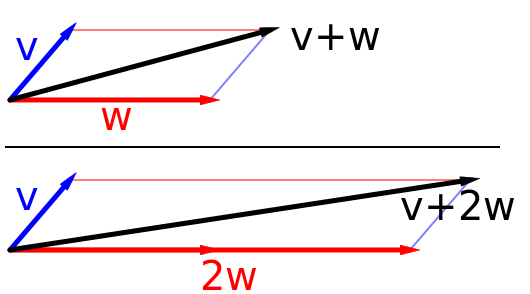
\includegraphics[width=.3\textwidth]{_img/Vector_add_scale.svg.png}
		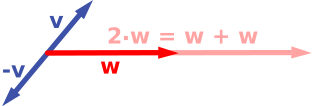
\includegraphics[width=.3\textwidth]{_img/Scalar_multiplication.svg.png}
	  \caption{Geometrical Meaning: Addition, Subtraction, and Scalar Multiplication}
	  \label{fig:_img_Vector_add_scale.svg}	
	\end{figure}
	
\end{frame}
%--- Next Frame ---%

\begin{frame}[t]{Scalar Multiplication}
	Let $r,s$ be scalars (or real numbers). $i.e.$, $r,s\in \mathbb{R}^1$.
	\begin{defn}
		[Scalar Multiplication]
		\[
			(r\mathbf{u})_i:= ru_i \quad\forall i
		\]
	\end{defn}
	Geometrically, scalar multiplcation means stretching or shrinking.
	
	\begin{block}
		{Algebraic Properties of Vector Operation}
		\begin{align*}
			\mathbf{u+v} &= \mathbf{v+u} \tag{Commutative Law}\\
			(r+s)\mathbf{u} &= r\mathbf{u}+s\mathbf{u} \tag{Distributive Law 1}\\
			r(\mathbf{u+v}) &= r\mathbf{u}+r\mathbf{v} \tag{Distributive Law 2}
		\end{align*}
	\end{block}
	In fact, any set of objects with a vector addition and scalar multiplication satisfying above laws is called \uline{vector space} and \uline{vector} is defined as the element of \uline{vector space}. (Vector is defined by operations and their laws)
\end{frame}

%--- Next Frame ---%
% section the_albevra_of_vectors (end)

\section{Length and Inner Product in $\mathbb{R}^n$} % (fold)
\label{sec:length_and_inner_product_in_mathbb_r_n}
\begin{frame}[t]{Length and Direction}
	\begin{defn}
		[Length of Vector $||\overrightarrow{\mathbf{pq}}||$]
		\[
			||\mathbf{\overrightarrow{pq}}|| := \sqrt{\sum_i^n (q_i-p_i)^2}
		\]
	\end{defn}
	\begin{thm}
		[10.1]\[
			||r\mathbf{v}||=|r|\cdot||\mathbf{v}|| \quad \forall r\in \mathbb{R}\land \forall\mathbf{v}\in\mathbb{R}^n
		\]
	\end{thm}
	Any vector has two kinds of information: (1) length, and  (2) direction. 
	\begin{defn}
		[Unit Vector (Direction of a vector)]
		\[
		\text{Unit vector of }\mathbf{v}:=\frac{\mathbf{v}}{||\mathbf{v}||}
		\]
	\end{defn}
\end{frame}
%--- Next Frame ---%

\begin{frame}[t]{The Inner Product}
	\begin{defn}
		[Euclidean Inner Product (or dot product)]
		\[
			\mathbf{u}\bullet\mathbf{v}:=\sum_i^n u_iv_i \in \mathbb{R}^1
		\]
	\end{defn}
	\begin{thm}
		[10.2: Properties of Inner Product]\begin{enumerate}
			\item $\mathbf{u\bullet v}=\mathbf{v\bullet u}$
			\item $\mathbf{u\bullet(v+w)}=\mathbf{u\bullet v + u\bullet w}$
			\item $\mathbf{u}\bullet(r\mathbf{v})=r(\mathbf{u\bullet v})=(r\mathbf{u})\bullet\mathbf{v}$
			\item $\mathbf{u\bullet u}\ge 0$
			\item $\mathbf{u\bullet u}=0\quad\iff\quad \mathbf{u}=\mathbf{0}$ 
			\item $\mathbf{(u+v)\bullet(u+v)=u\bullet u + 2 u\bullet v + v\bullet v}$
		\end{enumerate}
	\end{thm}
\end{frame}
%--- Next Frame ---%

\begin{frame}[t]{Inner Product and Angle between Two Vectors}
	\begin{thm}
		[10.3] Let $\theta$ be the angle between $\mathbf{u,v}$. Then, \[
			\mathbf{u\bullet v} = ||\mathbf{u}||\cdot||\mathbf{v}||\cos \theta
		\]
	\end{thm}
	\begin{thm}
		[10.4] \begin{enumerate}
			\item $\theta$ is acute if $\mathbf{u\bullet v}>0$
			\item $\theta$ is obtuse if $\mathbf{u\bullet v}<0$
			\item $\theta$ is right if $\mathbf{u\bullet v}=0$
		\end{enumerate}
	\end{thm}
	\begin{thm}
		[10.5: Triangle Inequality]
		\[
			||\mathbf{u+v}||\le ||\mathbf{u}||+||\mathbf{v}||
		\]\[
			\big| ||\mathbf{u}||-||\mathbf{v}|| \big|\le ||\mathbf{u-v}||
		\]
	\end{thm}
\end{frame}
%--- Next Frame ---%

\begin{frame}[t]{Norms}
	\begin{defn}[Norms]
		Any operation ($X$) of a vector to a real number satisfying below three properties is \uline{norm}. Length of vector is a norm. 
		\begin{enumerate}
			\item $X(\mathbf{u})\ge 0 \land X(\mathbf{u})=0$ only when $\mathbf{u}=\mathbf{0}$
			\item $X(r\mathbf{u})=|r|X(\mathbf{u})$
			\item $X(\mathbf{u+v})\le X(\mathbf{u})+X(\mathbf{v})$
		\end{enumerate}
	\end{defn}
	Norm is set of distance measures between two vectors. 
\end{frame}
%--- Next Frame ---%
% section length_and_inner_product_in_mathbb_r_n (end)

\section{Lines and Planes} % (fold)
\label{sec:lines}
\begin{frame}[t]{1D,2D Objects in $\mathbb{R}^n$ Spaces}
	\begin{block}
		{Lines:One dimensional objects in $\mathbb{R}^n$ Spaces}
		$\mathbf{x}$ representing a line passing $\overline{\mathbf{x_0}}$ with direction $\overline{\mathbf{v}}$ is:\[
			\mathbf{x} = \overline{\mathbf{x_0}}+t\overline{\mathbf{v}}\quad \forall t\in\mathbb{R} \tag{Parametric Representation}
		\]
		$\mathbf{x}$ representing a line passing $\overline{\mathbf{x_0}},\overline{\mathbf{x_1}}$ is: \[
			\mathbf{x} = (1-t)\overline{\mathbf{x_0}}+t\overline{\mathbf{x_1}}\quad\forall t\in\mathbb{R} \tag{Parametric Representation}
		\]
	\end{block}
	\begin{block}
		{Planes: Two dimensional objects in $\mathbb{R}^n$ Spaces}
		$\mathbf{x}$ representing a plane  passing $\overline{\mathbf{x_0}}$ with direction $\overline{\mathbf{v_1}}$ and $\overline{\mathbf{v_2}}$ is:\[
			\mathbf{x} = \overline{\mathbf{x_0}}+t_1\overline{\mathbf{v_1}}+t_2\overline{\mathbf{v_2}}\quad \forall t_i\in\mathbb{R} \tag{Parametric Representation}
		\]
		$\mathbf{x}$ representing a plane containing $\overline{\mathbf{x_0}},\overline{\mathbf{x_1}},\overline{\mathbf{x_2}}$ is: \[
			\mathbf{x} = (1-t_1-t_2)\overline{\mathbf{x_0}}+t_1\overline{\mathbf{x_1}}+t_2\overline{\mathbf{x_2}}\quad\forall t_i\in\mathbb{R} \tag{Parametric Representation}
		\]
	\end{block}
\end{frame}
%--- Next Frame ---%

\begin{frame}[t]{Nonparametric Equations}
	\begin{defn}
		[Normal Vector]
		A \uline{normal vector} $\bar{\mathbf{n}}$ of a $n$-dimensional object $\mathbf{X}$ is a vector which is perpendicular to any vectors in the object. Suppose $\mathbf{x}$, $\bar{\mathbf{p}}$ are location vectors in the object. Then, \[
			\bar{\mathbf{n}}\bullet(\mathbf{x}-\bar{\mathbf{p}})=0\quad \forall \mathbf{x,\bar{p}}\in\mathbf{X}
		\]
	\end{defn}
	\begin{block}
		{Finding Normal Vector}
		\begin{enumerate}
			\item For linearly independent vectors $\mathbf{u_i}$, solve below systems of equations satisfying \[
				\mathbf{n}\bullet\mathbf{u_i}=0 \quad\forall i
			\] 
			\item $\mathbf{n}=\mathbf{u} \times \mathbf{v}$ (Only for $\mathbb{R}^3$ space)
			\[
				\mathbf{u} \times \mathbf{v} := \left(\left|\begin{matrix}
					u_2 & u_3 \\ v_2 & v_3
				\end{matrix}\right|,-\left|\begin{matrix}
					u_1&u_3\\ v_1 & v_3 
				\end{matrix}\right|,\left|\begin{matrix}
					u_1&u_2\\v_1&v_2
				\end{matrix}\right|\right)
			\]
		\end{enumerate}
	\end{block}
\end{frame}
%--- Next Frame ---%

\begin{frame}[t]{Hyperplanes}
	\begin{defn}
		[Hyperplane]
		$n-1$ dimensional object in $\mathbb{R}^n$ space is a \uline{hyperplane} with normal vector $\bar{\mathbf{a}}$ if:\[
			\bar{a}_1 x_1+\bar{a}_2 x_2+\cdots\bar{a}_n x_n = \bar d
		\]or, \[
			\bar{\mathbf{a}}\bullet\mathbf{x}=\bar d
		\]
	\end{defn}
\end{frame}
%--- Next Frame ---%
% section lines (end)

\section{Economic Applications} % (fold)
\label{sec:economic_applications}
\begin{frame}[t]{Budget Constraint}
	\begin{defn}
		[Commodity Bundle, Price Vector, Budget Set]
		Let $x_i\ge 0$ be the quantity of $i$th commodity. 
		\[
			\mathbf{x}:=(x_1,\dots,x_n),\quad x_i \ge 0\quad\forall i \tag{Commodity Bundle}
		\]
		Let $p_i\ge 0$ be the price of $i$th commodity. \[
			\mathbf{p}:=(p_1,\cdots,p_n),\quad p_i \ge 0\quad\forall i \tag{Price Vector}
		\]
		Then \uline{budget set} $\mathbf{x}$ can be defined with given budget $\bar{I}$:\[
			\bar{\mathbf{p}}\bullet{\mathbf{x}}\le \bar I \tag{Budget Constraint}
		\]
	\end{defn}
\end{frame}
%--- Next Frame ---%
% section economic_applications (end)

\end{document}



		% Line passing $\overline{\mathbf{x_0}}$ with normal vector $\overline{\mathbf{n}}$ is: \[
		% 	(\mathbf{x}-\overline{\mathbf{x_0}})\bullet\overline{\mathbf{n}}=0 \tag{Nonparametric Representation}
		% \]